\documentclass[11pt]{article}

\usepackage[margin=1in]{geometry}
\usepackage{setspace}
\onehalfspacing
\usepackage{graphicx}
\graphicspath{report_images/}
\usepackage{appendix}
\usepackage{listings}
\usepackage{float}
\usepackage{multirow}
\usepackage{amsthm}
% The next three lines make the table and figure numbers also include section number
\usepackage{chngcntr}
\counterwithin{table}{section}
\counterwithin{figure}{section}
% Needed to make titling page without a page number
\usepackage{titling}

% DOCUMENT INFORMATION =================================================
\font\titleFont=cmr12 at 11pt
\title {{\titleFont ECEN 429: Introduction to Digital Systems Design Laboratory \\ North Carolina Agricultural and Technical State University \\ Department of Electrical and Computer Engineering}} % Declare Title
\author{\titleFont Reporter: Chris Cannon} % Declare authors
\date{\titleFont February 22, 2018}
% ======================================================================

\begin{document}

\begin{titlingpage}
\maketitle
\begin{center}
	Prelab 5
\end{center}
\end{titlingpage}

\section{Introduction}
The purpose of this prelab is to refresh the concepts of latches that we covered in class. We are refreshing these concepts by analyzing questions related to latches and VHDL implementations.

\section{Background, Design Solution, Results}
\subsection{Problem 1}

\subsubsection{Question 1}
Block 1 declares a component based on the AND GATE entity defined in Code (1).

\subsubsection{Question 2}
Block 2 declares a component based on the OR GATE entity defined in Code (2).

\subsection{Problem 2}
\begin{figure}
\begin{center}
	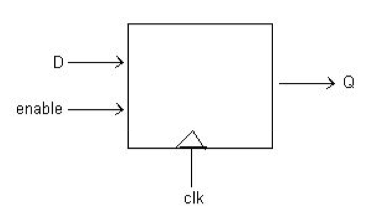
\includegraphics[width=0.5\textwidth]{./img5_1.png}
	\caption{\label{fig:dLatch}D Latch circuit diagram.}
\end{center}
\end{figure}

\subsubsection{Question 1}
Which line of code will give positive-edge triggered characteristics?
\begin{lstlisting}[language=VHDL]
if (clk’event) and (clk = ‘1’) then
\end{lstlisting}

\subsubsection{Question 2}
How does a D flip flop work?

A D flip flop will set the output value "Q" equal to the input "D" whenever it is both enabled and triggered by the appropriate clock edge, in the case of our latch above, the positive or rising clock edge. Otherwise, the output value "Q" remains unchanged.

\subsection{Problem 3}
\begin{figure}
\begin{center}
	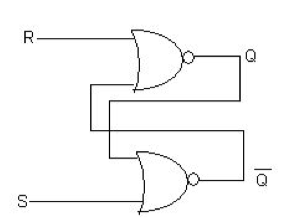
\includegraphics[width=0.5\textwidth]{./img5_2.png}
	\caption{\label{fig:srLatch}SR Latch circuit diagram.}
\end{center}
\end{figure}

\subsubsection{Problem 1}
Write the truth table for the SR Latch above.

\begin{table}[H]
\begin{center}
\begin{tabular}{| l | l | l | l | l |}
	\hline
	S & R & Q & Qnot & Comments\\ \hline
	0 & 0 & previous Q & previous Qnot & memory state \\ \hline
	0 & 1 & 0 & 1 & reset \\ \hline
	1 & 0 & 1 & 0 & set \\ \hline
	1 & 1 & \multicolumn{3}{|l|}{invalid input} \\ \hline
\end{tabular}
\end{center}
\end{table}

\subsubsection{Problem 2}
Write the code for the SR Latch.

\begin{lstlisting}[language=VHDL]
library IEEE;
use IEEE.STD_LOGIC_1164.ALL;

entity sr_latch is
    Port ( S, R : in STD_LOGIC;
           Q, notQ : inout STD_LOGIC);
end sr_latch;

architecture Behavioral of sr_latch is
signal notQ : STD_LOGIC;
begin

Q    <= R nor notQ;
notQ <= S nor Q;

end Behavioral;
\end{lstlisting}

\end{document}